\FloatBarrier
\subsection{Cyclic Similarity}\label{appen:additional_cyclic_similarity}

We include here additional plots to validate our cyclic similarity claims in \Cref{sec:cyclic_similarity}.

\Cref{fig:similar_residual_stream_cosine} complements \Cref{fig:similar_attention_patterns} by visualizing the cosine similarity between the residual streams after each layer for the range of Looped Transformers visualized in the original figure. Additional models (\raven{} and all retrofitted models) are visualized in \Cref{fig:similar_residual_stream_cosine} for 32 recurrences, demonstrating that the cyclic similarity is consistent for larger numbers of recurrences. We note that \raven{} continues its previous trend of all layer outputs converging to similar representations, with some cyclic similarity still visible. \Cref{fig:similar_attention_patterns_expanded} similarly provides an extended version of \Cref{fig:similar_attention_patterns}, demonstrating that attention matrix cyclic similarity holds to 32 recurrences.

\begin{figure*}[ht]
    \centering
    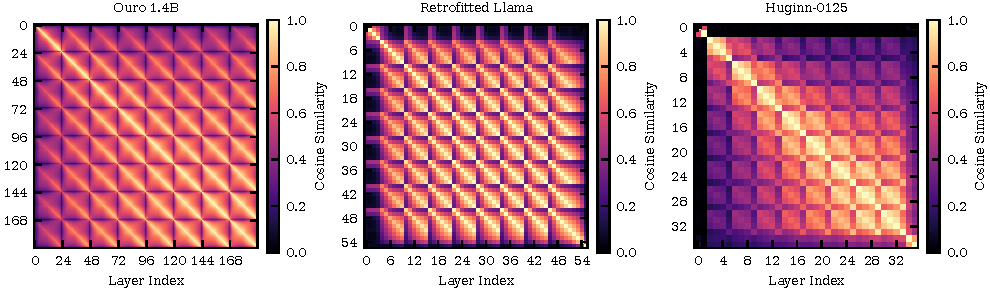
\includegraphics[width=0.9\linewidth]{figures/fixed_point/heatmaps/residual_stream_cosine_similarities.pdf}
    \vspace{-0.4cm}
    \caption{\textbf{Cosine similarity between residual streams after every pair of layers for different Transformer models}, averaged across the batch and sequence dimensions. \textbf{Left:} \ouro{} 1.4B \citep{zhu2025scaling}. \textbf{Center:} Retrofitted Llama \citep{mcleish2025teaching}. \textbf{Right:} \raven{} \citep{geiping2025scaling}. All models looped 8 times. Diagonal patterns indicate that the residual stream after each sub-block is most similar to the same block in the next recurrence; every layer in the recurrent block reaches a different fixed point.}
    \label{fig:similar_residual_stream_cosine}
\end{figure*}

\begin{figure}[ht]
    \centering
    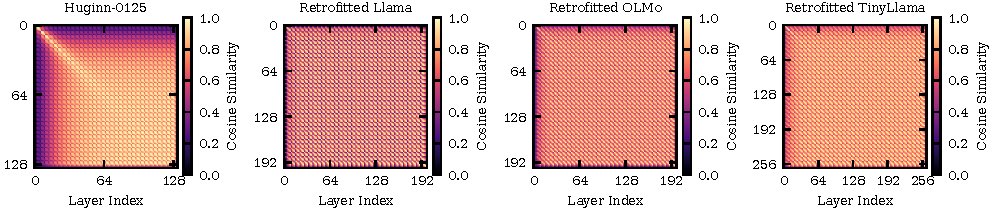
\includegraphics[width=\linewidth]{figures/fixed_point/heatmaps/residual_stream_cosine_similarities_expanded.pdf}
    \caption{Cosine similarity between residual streams after every pair of layers for different Transformer models, averaged across the batch and sequence dimensions. \textbf{Left:} \raven{} \citep{geiping2025scaling}. \textbf{Center Left:} Retrofitted Llama. \textbf{Center Right:} Retrofitted OLMo. \textbf{Right:} Retrofitted TinyLlama \citep{mcleish2025teaching}. All models looped 32 times. Extended version of \Cref{fig:similar_residual_stream_cosine}.}
    \label{fig:similar_residual_stream_cosine_expanded}
\end{figure}


\begin{figure}[ht]
    \centering
    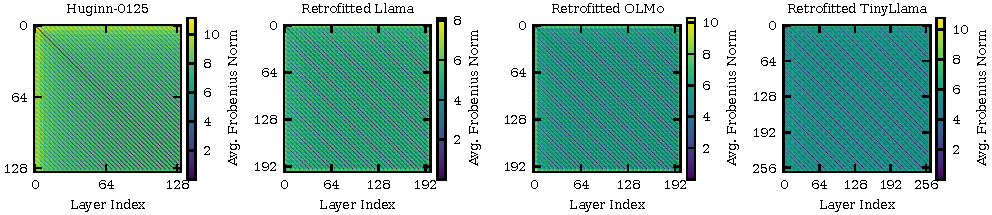
\includegraphics[width=\linewidth]{figures/fixed_point/heatmaps/attention_weight_norms_expanded.pdf}
    \caption{Frobenius norm between attention matrices for different Transformer models, averaged across the batch and head dimensions. \textbf{Left:} \raven{} \citep{geiping2025scaling}. \textbf{Center Left:} Retrofitted Llama. \textbf{Center Right:} Retrofitted OLMo. \textbf{Right:} Retrofitted TinyLlama \citep{mcleish2025teaching}. All models looped 32 times. Extended version of \Cref{fig:similar_attention_patterns}.}
    \label{fig:similar_attention_patterns_expanded}
\end{figure}

\FloatBarrier
\subsection{Fixed Point and Successive Differences}

In \Cref{sec:cyclic_similarity} we demonstrate that retrofitted Llama and \raven{} reach a fixed point but \ouro{} does not. We do so by -- for each layer -- computing an ``approximate fixed point'' after 128 recurrences and then plotting the norm of the difference for each layer at successive recurrences to this fixed point. In \Cref{fig:fixed_point_cosine_similarities} we demonstrate that this same behavior is observed when considering \emph{cosine similarity} to the fixed point, and in \Cref{fig:fixed_point_attention_differences} we see that it holds for attention matrices.

\begin{figure}[ht]
    \centering
    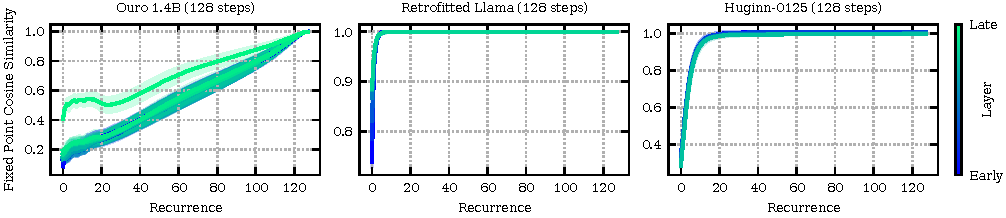
\includegraphics{figures/fixed_point/recurrencewise/fixed_point_cosine_similarities.pdf}
    \caption{\textbf{Cosine similarity between the residual stream after each layer in the recurrent block and its ``approximate fixed point''} - the residual stream after that layer in the 128th recursion. While \raven{} and retrofitted Llama quickly reach a fixed point, \ouro{} does not - even though the cosine similarity between successive recursions tends towards one, as evidenced by \Cref{fig:fixed_point_cosine_similarities}.}
    \label{fig:fixed_point_cosine_similarities}
\end{figure}

\begin{figure}[ht]
    \centering
    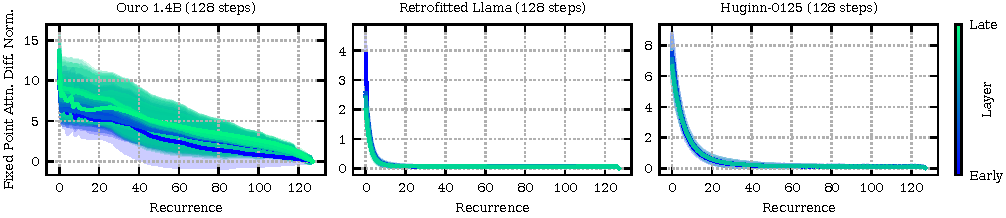
\includegraphics{figures/fixed_point/recurrencewise/fixed_point_attention_differences.pdf}
    \caption{\textbf{Frobenius norm between attention matrices of each layer in the recurrent block and their corresponding ``approximate fixed point''}; the attention matrices of the same layer in the 128th recursion. While \raven{} and retrofitted Llama quickly reach a fixed point, \ouro{} does not.}
    \label{fig:fixed_point_attention_differences}
\end{figure}

We then demonstrated in \Cref{fig:successive_norms} that all models, independent of whether they reach a strict fixed point or not, demonstrate converge towards very low difference norms between successive residual streams. We verify this same behavior holds for residual stream cosine similarities and attention matrix Frobenius norms in \Cref{fig:successive_cosine_similarities,fig:successive_attention_norms} respectively.

\begin{figure}[ht]
    \centering
    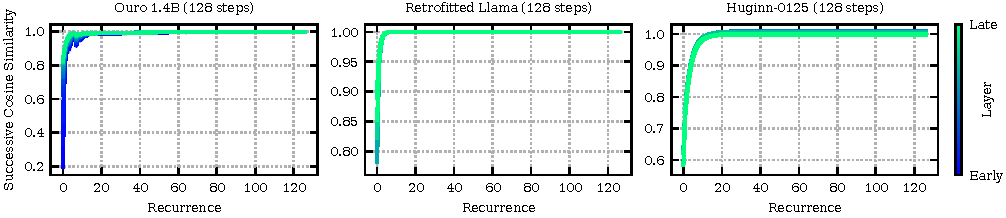
\includegraphics{figures/fixed_point/recurrencewise/successive_cosine_similarities.pdf}
    \caption{Cosine similarities between successive recursions of the residual stream after the same layer.}
    \label{fig:successive_cosine_similarities}
\end{figure}

\begin{figure}[ht]
    \centering
    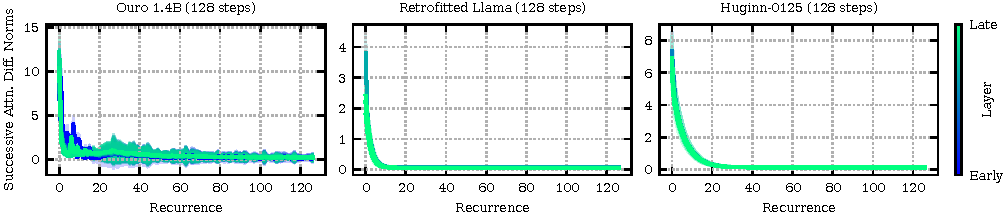
\includegraphics{figures/fixed_point/recurrencewise/successive_attention_differences.pdf}
    \caption{{Frobenius norm between attention matrices of each layer between successive recurrences.}}
    \label{fig:successive_attention_norms}
\end{figure}

\FloatBarrier
\subsection{Latent Space Trajectories}

In this section we visualize additional latent space trajectories, supplementing \Cref{fig:retro_llama_trajectory}. All trajectories are plotted by taking all latent states of the final token position on the test sequence described in \Cref{appen:experiment_details}, computing PCA on these latent state vectors and resultant dimensional reduction of this sequence of vectors. They are intended as illustrations to demonstrate qualitative behavior. \ouro{} is visualized in \Cref{fig:ouro_trajectory} and \raven{} in \Cref{fig:raven_trajectory}.

The \ouro{} trajectory is of particular interest as we are aware from the results in the main body of the paper that this model does not reach a strict fixed point. \Cref{fig:ouro_trajectory} demonstrates that -- on this test sequence -- \ouro{} reaches an approximately constant trajectory, but with visibly larger deviations even at later recurrences than \raven{} in \Cref{fig:raven_trajectory}.

However, we find evidence that this ``approximately stable trajectory'' behavior is not universal: for a simple ``maths'' test prompt (\texttt{The square root of 16 is}) shown in \Cref{fig:ouro_maths_trajectory}, \ouro{} appears to reach a stable trajectory in recurrences 8-16 before departing from this and appearing to become ``unstable''.

\begin{figure}[ht]
    \centering
    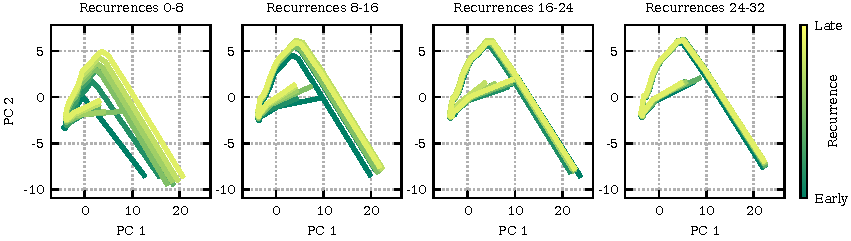
\includegraphics{figures/trajectory/pca_quartiles_Ouro_1.4B_32_steps_extended.pdf}
    \caption{\textbf{\ouro{} 1.4B \citep{zhu2025scaling} latent space trajectory} traced out by the hidden states of the final sequence position on the test prompt; reduced to two dimensions by computing PCA over all final sequence position embeddings.}
    \label{fig:ouro_trajectory}
\end{figure}

\begin{figure}[ht]
    \centering
    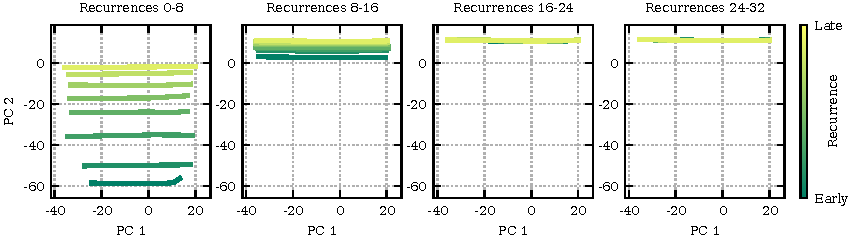
\includegraphics{figures/trajectory/pca_quartiles_Huginn-0125_32_steps_extended.pdf}
    \caption{\textbf{\raven{} \citep{geiping2025scaling} latent space trajectory} traced out by the hidden states of the final sequence position on the test prompt; reduced to two dimensions by computing PCA over all final sequence position embeddings.}
    \label{fig:raven_trajectory}
\end{figure}

\begin{figure}[ht]
    \centering
    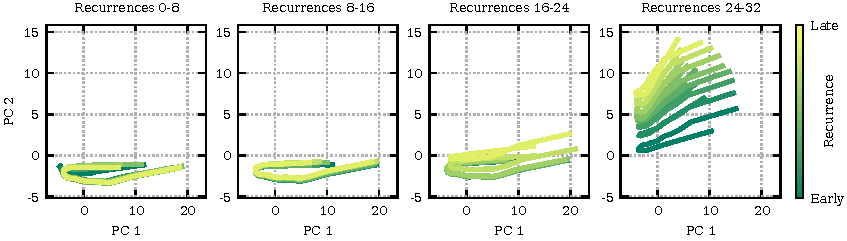
\includegraphics{figures/trajectory/maths_pca_quartiles_Ouro_1.4B_32_steps_extended.pdf}
    \caption{\textbf{\ouro{} 1.4B \citep{zhu2025scaling} latent space trajectory} traced out by the hidden states of the final sequence position on a ``maths'' test prompt (\texttt{The square root of 16 is}); reduced to two dimensions by computing PCA over all final sequence position embeddings.}
    \label{fig:ouro_maths_trajectory}
\end{figure}

\FloatBarrier
\subsection{Architecture Choices}

Here we provide more complete results to supplement \Cref{subsec:norm_and_ii}, visualizing fixed point difference norms and cosine similarities for various architecture choices in \Cref{fig:stability_initialised_fixed_point_norms,fig:stability_initialised_fixed_point_cosine_similarities} respectively.

\begin{figure}[ht]
    \centering
    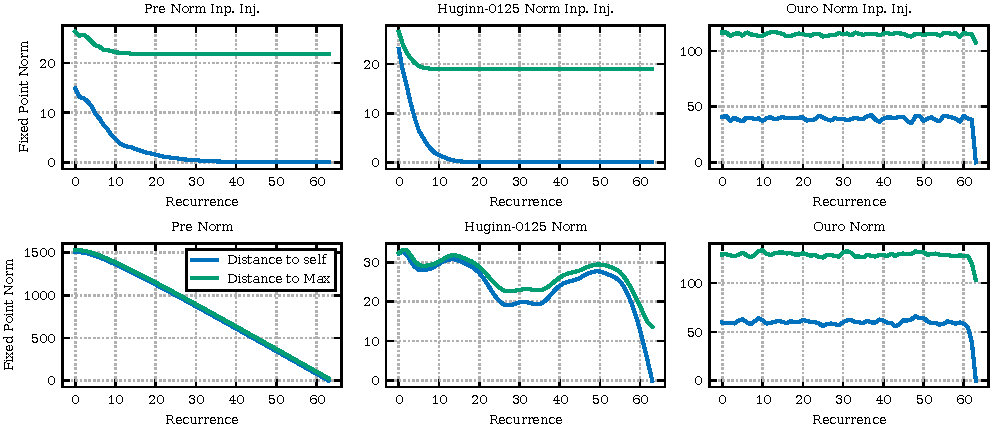
\includegraphics[width=0.8\linewidth]{figures/fixed_point/stability_initialised_fixed_point_norms.pdf}
    \caption{\textbf{Norm of the difference between the residual stream after the first layer in the recurrent block for successive recurrences and an ``approximate fixed point''} -- the residual stream in the 128th recurrence. Two fixed point differences are visualized: the difference to the fixed point of the same (first) layer (blue) and the difference to the fixed point which has the greatest norm difference from the first layer (green). Visualized are a range of norm structures (columns), with input injection (top row) and without (bottom row). All models are randomly initialized with 12 layers in the recurrent block, and no prelude or coda.}
    \label{fig:stability_initialised_fixed_point_norms}
\end{figure}

\begin{figure}[ht]
    \centering
    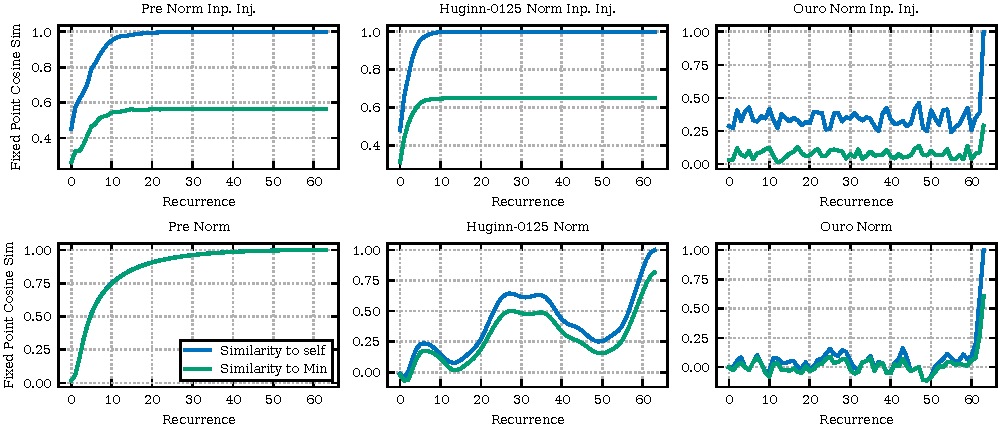
\includegraphics[width=0.8\linewidth]{figures/fixed_point/stability_initialised_fixed_point_cosine_similarities.pdf}
    \caption{\textbf{Cosine similarity between the residual stream after the first layer in the recurrent block for successive recurrences and an ``approximate fixed point''} -- the residual stream in the 128th recurrence. Two fixed point differences are visualized: the difference to the fixed point of the same (first) layer (blue) and the difference to the fixed point which has the lowest cosine similarity to the first layer (green). Visualized are a range of norm structures (columns), with input injection (top row) and without (bottom row). All models are randomly initialized with 12 layers in the recurrent block, and no prelude or coda.}
    \label{fig:stability_initialised_fixed_point_cosine_similarities}
\end{figure}

We also verify that the results presented are not particular to 12 layers by visualising results for both 4 and 16 layers in \Cref{fig:stability_initialised_fixed_point_cosine_similarities_multiple_layers}, showing qualitatively identical behavior.

\begin{figure}[ht]
    \centering
    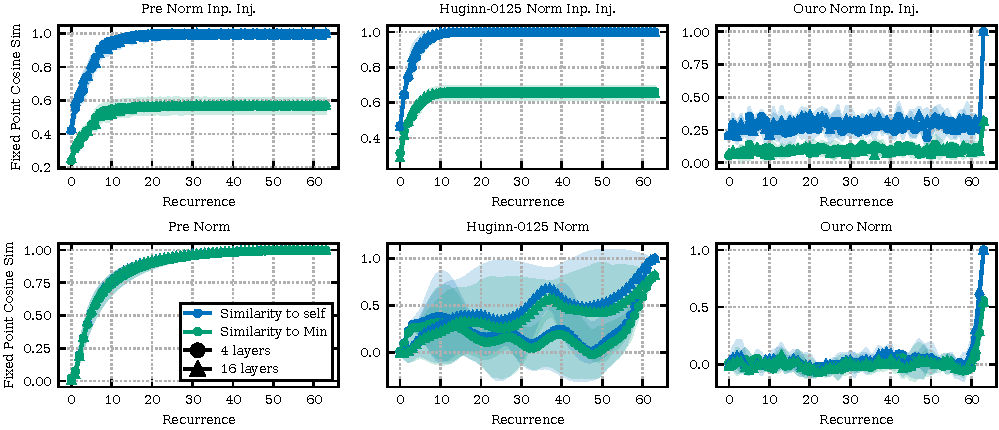
\includegraphics[width=0.8\linewidth]{figures/fixed_point/stability_initialised_final_state_difference_sim_multiple_layers.pdf}
    \caption{\textbf{Cosine similarity between the residual stream after the first layer in the recurrent block for successive recurrences and an ``approximate fixed point''} -- the residual stream in the 128th recurrence. Two fixed point differences are visualized: the difference to the fixed point of the same (first) layer (blue) and the difference to the fixed point which has the lowest cosine similarity to the first layer (green). Visualized are a range of norm structures (columns), with input injection (top row) and without (bottom row). Here models of 4 and 16 layers are compared, showing qualitatively identical behavior and demonstrating that the behavior is not particular to 12 layers.}
    \label{fig:stability_initialised_fixed_point_cosine_similarities_multiple_layers}
\end{figure}